% A0 portrait conference poster -- "Deep Tournament Selection for Genetic Algorithms" (PPSN 2026)
% Build: export PATH="/Library/TeX/texbin:$PATH" && latexmk -pdf poster.tex
\documentclass[final]{beamer}
\usepackage[size=a0,orientation=portrait,scale=1.30]{beamerposter}
\usepackage[T1]{fontenc}
\usepackage{lmodern}
\usepackage{amsmath,amssymb}
\usepackage{graphicx}
\usepackage{booktabs}
\usepackage{tikz}
\usetikzlibrary{positioning, shapes.geometric, arrows.meta, fit, backgrounds, calc, shapes.misc}
\usepackage{tcolorbox}
\tcbuselibrary{skins}
\usepackage{fontawesome5}
\usepackage{qrcode}
\usepackage{colortbl}

%==================== Palette ====================
\definecolor{bguBlue}{RGB}{20,52,124}     % deep navy header bars / title
\definecolor{bguMid}{RGB}{0,99,168}        % mid blue accents
\definecolor{cardBlue}{RGB}{244,247,252}   % light card background
\definecolor{learnPurple}{RGB}{124,99,196} % learned modules
\definecolor{compGreen}{RGB}{36,150,98}    % computation / decision
\definecolor{ink}{RGB}{30,38,52}           % body text

%==================== Operator Colors for Legend ====================
\definecolor{colorRoulette}{HTML}{FF7F00}    % Orange
\definecolor{colorSUS}{HTML}{00C5CD}         % Cyan
\definecolor{colorLinearRank}{HTML}{1F78B4}  % Blue
\definecolor{colorTruncation}{HTML}{E31A1C}  % Red
\definecolor{colorTournament}{HTML}{737373}  % Grey
\definecolor{colorSODGA}{HTML}{A65628}       % Brown
\definecolor{colorDTS}{HTML}{5E3C99}         % Purple

\definecolor{gcBg}{RGB}{240,244,250}       % Graph Coloring fill
\definecolor{scBg}{RGB}{240,248,242}       % Set Cover fill
\definecolor{tspBg}{RGB}{254,246,238}      % TSP fill
\setbeamercolor{background canvas}{bg=white}
\setbeamercolor{normal text}{fg=ink}
\usebeamercolor*{normal text}
\setbeamertemplate{navigation symbols}{}
\setbeamertemplate{itemize items}{\textcolor{bguMid}{\textbf{--}}}
\setbeamercolor{itemize item}{fg=bguMid}
\setbeamercolor{itemize subitem}{fg=bguMid}

%==================== Poster font scale (Unified Large A0 Print Scale) ====================
\newcommand{\FSHeader}{\fontsize{72}{82}\selectfont}     % Poster Title
\newcommand{\FSAuthor}{\fontsize{36}{42}\selectfont}     % Authors
\newcommand{\FSSection}{\fontsize{33}{39}\selectfont}    % Section Headers (card titles)
\newcommand{\FSSubhead}{\fontsize{26}{32}\selectfont}    % Main Subheadings / Captions
\newcommand{\FSBody}{\fontsize{24.5}{30.5}\selectfont}   % General Body Text (Motivation, Core Idea, Method Overview points, etc.)
\newcommand{\FSDetails}{\fontsize{22.5}{26.5}\selectfont}% Details / Subtitles / Card Points
\newcommand{\FSNotes}{\fontsize{19.5}{23.5}\selectfont}  % Footnotes / Small Notes / Takeaways / Legends

%==================== Poster rhythm ====================
\newcommand{\PosterSectionGap}{0.10cm}
\newcommand{\PosterSubheadGap}{2mm}

% Standardized Subheading Commands
\newcommand{\postersubhead}[1]{{\color{bguBlue}\FSSubhead\bfseries #1}\par\vspace{\PosterSubheadGap}}
\newcommand{\postersubheadcenter}[1]{{\centering\color{bguBlue}\FSSubhead\bfseries #1\par}\vspace{\PosterSubheadGap}}
\newcommand{\postersubsubhead}[1]{{\FSSubhead\bfseries #1}\par\vspace{1.5mm}}

%==================== Section boxes & components ====================
\newtcolorbox{secbox}[2][]{
  enhanced, colback=white, colframe=bguBlue, boxrule=0.5mm, arc=2.5mm,
  top=4.5mm, bottom=4.5mm, left=7mm, right=7mm,
  title={#2}, fonttitle=\FSSection\bfseries, coltitle=white, colbacktitle=bguBlue,
  halign title=center, toptitle=2.5mm, bottomtitle=2.5mm,
  #1
}

\newtcolorbox{takeawaybox}{
  enhanced, arc=2mm, colback=bguMid!8, colframe=bguMid!50, boxrule=0.5mm,
  left=4mm, right=4mm, top=2.5mm, bottom=2.5mm, halign=center,
}

\newtcolorbox{trophybox}{
  enhanced, arc=3mm, colback=bguMid!10, colframe=bguMid, boxrule=0.7mm,
  left=6mm, right=6mm, top=3.5mm, bottom=3.5mm,
}

\newcommand{\leftcompactitem}[2]{%
  \par\vspace{2.0mm}\noindent
  \begin{minipage}[c]{0.11\linewidth}\centering\textcolor{bguMid}{\fontsize{27}{27}\selectfont #1}\end{minipage}%
  \hfill
  \begin{minipage}[c]{0.86\linewidth}\raggedright\FSBody #2\end{minipage}\par\vspace{2.0mm}}

\newcommand{\sectiongap}{\vspace{\PosterSectionGap}}
\newcommand{\projecturl}{https://github.com/EC-KitY/DTS-for-GA}

\newcommand{\MethodOverviewTikZ}{%
\begin{tikzpicture}[
    x=1.75cm, y=1cm,
    >=Stealth, font=\fontsize{12}{14.5}\selectfont\sffamily,
    learned/.style={rectangle, rounded corners, draw=learnPurple!75, fill=learnPurple!16, align=center, very thick, inner sep=2.2mm},
    comp/.style={rectangle, rounded corners, draw=compGreen!75, fill=compGreen!16, align=center, very thick, inner sep=2.2mm},
    plus/.style={circle, draw=black!60, fill=gray!18, thick, inner sep=1pt, font=\fontsize{14}{14}\selectfont},
    tourn/.style={rectangle, rounded corners=4mm, draw=bguMid!40, thick, fill=bguMid!5, inner xsep=15pt, inner ysep=9pt}
]
    \node[font=\fontsize{13.5}{15}\selectfont\bfseries] at (3.0,5.1) {(1)};
    \node[font=\fontsize{13.5}{15}\selectfont\bfseries] at (8.0,5.1) {(2)};
    \node[font=\fontsize{13.5}{15}\selectfont\bfseries] at (12.9,5.1) {(3)};
 
    \node[font=\fontsize{13.5}{15}\selectfont\bfseries] (T1_title) at (5.6, 3.5) {Tournament $T_1$};
    \node[learned] (enc_ind_1) at (0, 2.5) {Embedding \\ Individuals \\ $Enc_{\theta}$};
    \node[learned] (enc_rank_1) at (0, 0.5) {Embedding \\ Global \& \\ Local Ranks};
    \node[plus] (plus_1) at (2.0, 1.5) {$+$};
    \draw[->, thick] (enc_ind_1.east) -| (plus_1.north);
    \draw[->, thick] (enc_rank_1.east) -| (plus_1.south);
    \node[comp] (h_1) at (4.2, 1.5) {$\left\{ \begin{aligned} &\tilde{H}_{1,j} = H_i + {} \\ &e_{r_i} + e^{\text{local}}_{r_{1,j}} \end{aligned} \right\}$};
    \draw[->, thick] (plus_1) -- (h_1);
    \node[learned] (cte_1) at (7.6, 1.5) {Contextual \\ Tournament \\ Evaluation};
    \draw[->, thick] (h_1) -- (cte_1);
    \node[comp,font=\fontsize{13}{13}\selectfont] (pi_1) at (9.4, 1.5) {$\pi_1$};
    \draw[->, thick] (cte_1) -- (pi_1);
    \node[learned] (sample_1) at (11.4, 1.5) {Sample \\[-1mm] $a_1 \sim \pi_1$};
    \draw[->, thick] (pi_1) -- (sample_1);
 
    \node[font=\fontsize{13.5}{15}\selectfont\bfseries] (Tn_title) at (5.6, -3.2) {Tournament $T_N$};
    \node[learned] (enc_ind_n) at (0, -4.2) {Embedding \\ Individuals \\ $Enc_{\theta}$};
    \node[learned] (enc_rank_n) at (0, -6.2) {Embedding \\ Global \& \\ Local Ranks};
    \node[plus] (plus_n) at (2.0, -5.2) {$+$};
    \draw[->, thick] (enc_ind_n.east) -| (plus_n.north);
    \draw[->, thick] (enc_rank_n.east) -| (plus_n.south);
    \node[comp] (h_n) at (4.2, -5.2) {$\left\{ \begin{aligned} &\tilde{H}_{N,j} = H_i + {} \\ &e_{r_i} + e^{\text{local}}_{r_{N,j}} \end{aligned} \right\}$};
    \draw[->, thick] (plus_n) -- (h_n);
    \node[learned] (cte_n) at (7.6, -5.2) {Contextual \\ Tournament \\ Evaluation};
    \draw[->, thick] (h_n) -- (cte_n);
    \node[comp,font=\fontsize{13}{13}\selectfont] (pi_n) at (9.4, -5.2) {$\pi_N$};
    \draw[->, thick] (cte_n) -- (pi_n);
    \node[learned] (sample_n) at (11.4, -5.2) {Sample \\[-1mm] $a_N \sim \pi_N$};
    \draw[->, thick] (pi_n) -- (sample_n);
 
    \node[comp,font=\fontsize{12}{14}\selectfont] (new_pop) at (14.4, -1.25) {New \\ Population};
    \node[learned,font=\fontsize{12}{14}\selectfont] (pg) at (14.4, -4.7) {Policy \\ Gradient \\ Update};
    \draw[->, thick] (sample_1.east) to[out=0, in=90] (new_pop.north);
    \draw[->, thick] (sample_n.east) to[out=0, in=180] (new_pop.west);
    \draw[->, thick] (new_pop.south) -- (pg.north);
 
    \draw[->, thick, dashed] (pg.south) .. controls +(0, -1.2) and +(0, -1.2) .. (cte_n.south);
    \draw[->, thick, dashed] (pg.south) .. controls +(0, -2.6) and +(0.5, -0.5) .. (enc_rank_n.south east);
    \draw[->, thick, dashed] (pg.south) .. controls +(0, -3.5) and +(3.0, 0) .. (5.0, -7.8)
        .. controls +(-2.0, 0) and +(0, -1.0) .. (1.6, -5.6) -- (enc_ind_n.south east);
    \draw[->, thick, dashed] (pg.west) .. controls +(-1.5, 0) and +(0, -1.5) .. (12.6, -1.5) .. controls +(0, 1.5) and +(0, -1.5) .. (cte_1.south);
    \draw[->, thick, dashed] (pg.west) .. controls +(-1.5, 0) and +(0, -1.0) .. (12.8, -1.3) .. controls +(0, 1.0) and +(2.0, 0) .. (6, 0.0) .. controls +(-2.0, 0) and +(0.5, -0.4) .. (enc_rank_1.south east);
    \draw[->, thick, dashed] (pg.west) .. controls +(-1.5, 0) and +(0, -1.0) .. (13.0, -1.4)
        .. controls +(0, 0.5) and +(3.0, 0) .. (5.0, -0.2)
        .. controls +(-2.0, 0) and +(0, -1.0) .. (1.6, 1.1) -- (enc_ind_1.south east);
 
    \node[font=\fontsize{18}{18}\selectfont] at (2.0, -1.85) {$\vdots$};
    \node[font=\fontsize{18}{18}\selectfont] at (7.6, -1.85) {$\vdots$};
    \node[font=\fontsize{18}{18}\selectfont] at (11.4, -1.85) {$\vdots$};
 
    \begin{scope}[on background layer]
        \node[tourn, fit=(enc_ind_1) (sample_1) (enc_rank_1) (T1_title)] {};
        \node[tourn, fit=(enc_ind_n) (sample_n) (enc_rank_n) (Tn_title)] {};
    \end{scope}
    \draw[dashed, thick, gray] (5.9, 5.3) -- (5.9, -7.2);
    \draw[dashed, thick, gray] (10.4, 5.3) -- (10.4, -7.2);
\end{tikzpicture}%
}

\newcommand{\OnlinePolicyTikZ}{%
\begin{tikzpicture}[
    x=1.12cm, y=1cm,
    >=Stealth, font=\fontsize{12}{14.5}\selectfont\sffamily,
    stepnode/.style={rectangle, rounded corners=2mm, draw=bguMid!40, fill=cardBlue, align=center, very thick, inner sep=1.8mm, minimum width=2.4cm, minimum height=2.8cm},
    arrowstyle/.style={->, very thick, bguBlue}
]
    % Nodes (evenly spaced at x = 0, 2.95, 5.90, 8.85, 11.80 for equal arrow lengths)
    \node[stepnode] (n1) at (0, 0) {
        \textcolor{bguMid}{\fontsize{25}{25}\selectfont\faUsers}\\[2mm]
        \textbf{Population}\\
        $P_t$
    };
    \node[stepnode] (n2) at (2.8, 0) {
        \textcolor{bguMid}{\fontsize{25}{25}\selectfont\faTrophy}\\[2mm]
        \textbf{Policy-based}\\
        \textbf{sampling}
    };
    \node[stepnode] (n3) at (5.6, 0) {
        \textcolor{bguMid}{\fontsize{25}{25}\selectfont\faDna}\\[2mm]
        \textbf{Generate}\\
        $P_{t+1}$
    };
    \node[stepnode] (n4) at (8.7, 0) {
        \textcolor{bguMid}{\fontsize{25}{25}\selectfont\faChartLine}\\[2mm]
        \textbf{Calculate}\\
        \textbf{reward}
    };
    \node[stepnode] (n5) at (11.8, 0) {
        \textcolor{bguMid}{\fontsize{25}{25}\selectfont\faSync}\\[2mm]
        \textbf{REINFORCE}\\
        \textbf{policy update}
    };

    % Connections (equal length arrows)
    \draw[arrowstyle] (n1) -- (n2);
    \draw[arrowstyle] (n2) -- (n3);
    \draw[arrowstyle] (n3) -- (n4);
    \draw[arrowstyle] (n4) -- (n5);

    % Feedback loop (smooth circular arc)
    \draw[->, very thick, dashed, bguBlue] (n5.south) .. controls +(0, -2.2) and +(0, -2.2) .. (n1.south);
\end{tikzpicture}%
}

%==================== Header ====================
\setbeamertemplate{headline}{
  \vspace{1.0cm}
  \begin{columns}[c,onlytextwidth]
    \begin{column}{0.29\paperwidth}
      
\includegraphics[width=\linewidth]{images/stein_logo.png}
    \end{column}
    \begin{column}{0.43\paperwidth}
      \centering
      {\color{bguBlue}\FSHeader\bfseries Deep Tournament Selection}\\[6mm]
      {\color{bguBlue}\FSHeader\bfseries for Genetic Algorithms}\\[10mm]
      {\color{ink}\FSAuthor Eliad Shem-Tov\textsuperscript{$\star$}\quad Ron Edri\textsuperscript{$\star$}\quad Achiya Elyasaf}\\[4mm]
      {\color{bguMid}\FSBody\itshape \textsuperscript{$\star$}Equal contribution}
    \end{column}
    \begin{column}{0.21\paperwidth}
      \hspace*{-1.8cm}%
      \begin{minipage}{0.19\paperwidth}
        \raggedleft
        
\includegraphics[height=5.5cm]{images/logo-pstn.png}
      \end{minipage}
    \end{column}
  \end{columns}
  \vspace{0.7cm}
  \hspace*{0.02\paperwidth}\textcolor{bguBlue}{\rule{0.96\paperwidth}{1.4mm}}
}

\begin{document}
\begin{frame}[t]
\vspace{-0.8cm}

%================================================================
% ROW 1: TOP BLOCK (Motivation + Core Idea + Contributions = Method Overview)
%================================================================
\begin{columns}[t,onlytextwidth]

\begin{column}{0.370\paperwidth}
\begin{secbox}{1. MOTIVATION}
\FSBody
\begin{itemize}\setlength\itemsep{2.5mm}
  \item Selection drives the \textbf{exploration--exploitation} balance in GAs.
  \item Existing selection rules are mostly \textbf{static} and \textbf{handcrafted}.
  \item There are learning-based crossover and mutation operators. Selection has largely been left behind.
\end{itemize}
\end{secbox}

\sectiongap

\begin{secbox}{2. CORE IDEA}
\FSBody
\begin{itemize}\setlength\itemsep{2.5mm}
  \item Learn a \textbf{probability distribution} over tournament candidates.
  \item Train tournament selection online as a \textbf{Markov Decision Process (MDP)}, with \textbf{no extra fitness evaluations}.
  \item Use \textbf{Transformer self-attention} with global and local ranks to adapt \textbf{selection pressure}.
\end{itemize}
\end{secbox}

\sectiongap

\begin{secbox}{3. CONTRIBUTIONS}
\FSBody
\begin{itemize}\setlength\itemsep{2.5mm}
  \item Introduce \textbf{Deep Tournament Selection (DTS)}, a domain-independent operator that learns tournament-selection decisions.
  \item Propose a \textbf{Contextual Tournament Evaluation} architecture combining Transformer embeddings, global and local rank encodings, and a self-attention pointer mechanism.
  \item Design a \textbf{fully online training strategy} that interleaves optimization with the GA loop. We empirically demonstrate that this adapts selection pressure to achieve \textbf{faster convergence} and \textbf{better final quality} across Graph Coloring, Set Cover, and TSP with \textbf{negligible overhead}.
\end{itemize}
\end{secbox}
\end{column}

\hfill

\begin{column}{0.570\paperwidth}
\begin{secbox}{4. METHOD OVERVIEW}
\begin{minipage}[t][28.23cm][s]{\linewidth}
\centering
\vspace{1mm}
\resizebox{0.92\linewidth}{!}{\MethodOverviewTikZ}
\begin{tcolorbox}[enhanced,colback=cardBlue,colframe=bguMid!40,boxrule=0.35mm,arc=2mm,
    left=4mm,right=4mm,top=2mm,bottom=2mm,width=0.94\linewidth]
\centering\FSNotes
\tikz[baseline=-0.6ex]\node[rectangle,rounded corners=1mm,draw=learnPurple!75,fill=learnPurple!16,minimum width=8mm,minimum height=5mm]{};~Learned module
\hspace{6mm}
\tikz[baseline=-0.6ex]\node[rectangle,rounded corners=1mm,draw=compGreen!75,fill=compGreen!16,minimum width=8mm,minimum height=5mm]{};~Computation / decision
\hspace{6mm}
\tikz[baseline=-0.6ex]\draw[->,very thick] (0,0)--(0.9,0);~Data flow
\hspace{6mm}
\tikz[baseline=-0.6ex]\draw[->,very thick,dashed] (0,0)--(0.9,0);~Feedback / update
\end{tcolorbox}
\vfill
\begin{minipage}{0.96\linewidth}
\FSBody
\begin{minipage}[t]{0.32\linewidth}\raggedright\textbf{(1)} Embed each individual and add global \& local rank encodings.\end{minipage}\hfill
\begin{minipage}[t]{0.32\linewidth}\raggedright\textbf{(2)} Evaluate the tournament jointly to obtain a selection policy $\pi$.\end{minipage}\hfill
\begin{minipage}[t]{0.32\linewidth}\raggedright\textbf{(3)} Sample a winner; elite-fitness gain rewards an online policy update.\end{minipage}
\end{minipage}
\vspace{1mm}
\end{minipage}
\end{secbox}
\end{column}

\end{columns}

\sectiongap

%================================================================
% ROW 2: MIDDLE BLOCK (How DTS Learns + Experimental Setup = Results)
%================================================================
\begin{columns}[t,onlytextwidth]

\begin{column}{0.370\paperwidth}
\begin{secbox}{5. HOW DTS LEARNS}
\FSBody
DTS treats tournament selection as a \textbf{Markov Decision Process} and learns the selection policy online using \textbf{REINFORCE}.
\vspace{6mm}

\postersubhead{Online policy optimization}

\begin{center}
  \resizebox{0.86\linewidth}{!}{\OnlinePolicyTikZ}
\end{center}

\postersubhead{MDP formulation}
\begin{itemize}\setlength\itemsep{3mm}
  \item \textbf{State:} Current population $P_t$ with fitness values.
  \item \textbf{Action:} Select one individual from each tournament.
  \item \textbf{Policy:} Deep selection model (see \textbf{Method Overview} for more details).
  \item \textbf{Reward:} Improvement in the average top-5 fitness between consecutive generations:
\end{itemize}
\vspace{5mm}
\[
R_t = \frac{1}{m}\left(\sum_{f \in f_{t+1}^{(m)}} f - \sum_{f \in f_t^{(m)}} f\right), \quad m=5
\]
\vspace{4.5mm}

\postersubhead{Online training}
\begin{itemize}\setlength\itemsep{3mm}
  \item Policy updates are performed online using \textbf{REINFORCE}.
  \item Uses fitness values already produced during evolution, requiring \textbf{no additional fitness evaluations}.
  \item Model updates are performed every \textbf{10 generations}.
\end{itemize}
\end{secbox}

\sectiongap

\begin{secbox}{6. EXPERIMENTAL SETUP}
\FSBody
\postersubhead{Benchmark domains}
\vspace{4mm}
\leftcompactitem{\faProjectDiagram}{\textbf{Graph Coloring}: Minimize the number of colors while ensuring adjacent vertices receive different colors.}
\vspace{2mm}
\leftcompactitem{\faTasks}{\textbf{Set Cover}: Minimize selected subsets while ensuring all universe elements are covered.}
\vspace{2mm}
\leftcompactitem{\faRoute}{\textbf{Traveling Salesman Problem (TSP)}: Minimize tour length over valid city permutations.}

\vspace{6mm}
\postersubhead{Baseline selection operators}
\vspace{1.5mm}
\leftcompactitem{\faChartPie}{\textbf{Fitness-based}: Roulette selection; Stochastic Universal Sampling (SUS).}
\vspace{2mm}
\leftcompactitem{\faSortAmountUp}{\textbf{Rank-based}: Linear rank; Truncation.}
\vspace{2mm}
\leftcompactitem{\faTrophy}{\textbf{Competition-based}: Tournament.}
\vspace{2mm}
\leftcompactitem{\faRandom}{\textbf{Adaptive}: Selection operator decider genetic algorithm (SODGA).}

\vspace{6mm}
\postersubhead{Comparison protocol}
\vspace{2mm}
\leftcompactitem{\faClipboardCheck}{\textbf{Evaluation:} Each baseline selection operator is run on all benchmark problems, with 15 runs per instance; statistical significance is assessed.}
\vspace{2mm}
\leftcompactitem{\faBullseye}{\textbf{Fairness comparison:} Identical GA parameters and budgets are used, with the selection operator being the only variation.}
\end{secbox}
\end{column}

\hfill

\begin{column}{0.570\paperwidth}
\begin{secbox}{7. RESULTS}
\vspace{1mm}
\postersubheadcenter{1. Final solution quality* (average over 15 runs; lower is better)}
\vspace{2mm}
\centering
\FSBody
\setlength{\tabcolsep}{8.5pt}
\renewcommand{\arraystretch}{1.3}
\begin{tabular}{clccccc>{\columncolor{cardBlue}}c}
\toprule
 & \textbf{Instance} & \textbf{SUS} & \textbf{Linear Rank} & \textbf{Truncation} & \textbf{Tournament} & \textbf{SODGA} & \multicolumn{1}{>{\columncolor{cardBlue}}c}{\textbf{DTS (ours)}} \\
\midrule
\raisebox{-1.3cm}[0pt][0pt]{\begin{tabular}{c} \fontsize{20}{24}\selectfont\bfseries Graph \\ \fontsize{20}{24}\selectfont\bfseries Coloring \\ \fontsize{15}{18}\selectfont (8 instances) \end{tabular}}
& games120   & 41.0 (1.7) & 43.2 (2.3) & 28.6 (1.2) & 34.7 (2.2) & 33.7 (2.3) & \textbf{25.0} (2.2) \\
& myciel7    & 76.3 (2.4) & 82.7 (3.2) & 59.7 (2.0) & 64.1 (2.4) & 63.1 (2.1) & \textbf{46.3} (5.4) \\
& \multicolumn{1}{c}{$\vdots$} & \multicolumn{1}{c}{$\vdots$} & \multicolumn{1}{c}{$\vdots$} & \multicolumn{1}{c}{$\vdots$} & \multicolumn{1}{c}{$\vdots$} & \multicolumn{1}{c}{$\vdots$} & \multicolumn{1}{>{\columncolor{cardBlue}}c}{\textbf{$\vdots$}} \\
& zeroin.i.2 & 92.3 (3.1) & 97.6 (2.7) & 73.1 (2.5) & 75.0 (2.6) & 74.0 (2.7) & \textbf{64.0} (2.6) \\
\addlinespace[2mm]
\midrule
\addlinespace[2mm]
\raisebox{-1.3cm}[0pt][0pt]{\begin{tabular}{c} \fontsize{20}{24}\selectfont\bfseries Set Cover \\ \fontsize{15}{18}\selectfont (8 instances) \end{tabular}}
& scp41      & 301.2 (23.2) & 257.2 (11.6) & 176.7 (29.2) & 74.2 (3.7) & 87.3 (4.9) & \textbf{67.5} (2.8) \\
& scp51      & 657.7 (45.9) & 597.6 (14.4) & 353.0 (63.3) & 130.0 (9.4) & 125.8 (6.4) & \textbf{99.6} (9.5) \\
& \multicolumn{1}{c}{$\vdots$} & \multicolumn{1}{c}{$\vdots$} & \multicolumn{1}{c}{$\vdots$} & \multicolumn{1}{c}{$\vdots$} & \multicolumn{1}{c}{$\vdots$} & \multicolumn{1}{c}{$\vdots$} & \multicolumn{1}{>{\columncolor{cardBlue}}c}{\textbf{$\vdots$}} \\
& scp65      & 265.5 (30.6) & 223.0 (9.3) & 98.4 (19.1) & 43.5 (2.5) & 41.3 (2.2) & \textbf{38.6} (1.7) \\
\addlinespace[2mm]
\midrule
\addlinespace[2mm]
\raisebox{-1.3cm}[0pt][0pt]{\begin{tabular}{c} \fontsize{20}{24}\selectfont\bfseries TSP \\ \fontsize{15}{18}\selectfont (8 instances) \\ \fontsize{15}{18}\selectfont ($\times 10^3$) \end{tabular}}
& berlin52   & 7.66 (0.13) & 7.78 (0.20) & 8.00 (0.19) & 8.00 (0.18) & 7.76 (0.10) & \textbf{7.56} (0.04) \\
& lin105     & 14.89 (0.07) & 15.26 (0.34) & 15.66 (0.69) & 15.22 (0.35) & 15.23 (0.29) & \textbf{14.65} (0.07) \\
& \multicolumn{1}{c}{$\vdots$} & \multicolumn{1}{c}{$\vdots$} & \multicolumn{1}{c}{$\vdots$} & \multicolumn{1}{c}{$\vdots$} & \multicolumn{1}{c}{$\vdots$} & \multicolumn{1}{c}{$\vdots$} & \multicolumn{1}{>{\columncolor{cardBlue}}c}{\textbf{$\vdots$}} \\
& att48      & 10.78 (0.14) & 10.81 (0.11) & 11.19 (0.24) & 10.96 (0.25) & 10.76 (0.09) & \textbf{10.70} (0.05) \\
\bottomrule
\end{tabular}\par
\vspace{5mm}
{\centering\FSNotes\itshape *Roulette Wheel selection underperformed consistently across all domains and was omitted for brevity.\par}
\vspace{2.5mm}

\begin{takeawaybox}
  \FSNotes\bfseries\color{bguBlue} DTS achieves the best or tied-best final objective on every benchmark instance
\end{takeawaybox}
\vspace{6mm}

\postersubheadcenter{2. Mean wall-clock time per generation (averaged over all instances; seconds)}
\vspace{2mm}
\centering
\FSBody
\setlength{\tabcolsep}{9pt}
\renewcommand{\arraystretch}{1.3}
\begin{tabular}{lcccccc>{\columncolor{cardBlue}}c}
\toprule
\textbf{Domain} & \textbf{Roulette Wheel} & \textbf{SUS} & \textbf{Linear Rank} & \textbf{Truncation} & \textbf{Tournament} & \textbf{SODGA} & \multicolumn{1}{>{\columncolor{cardBlue}}c}{\textbf{DTS (ours)}} \\
\midrule
Graph Coloring & 0.05 & 0.05 & 0.05 & 0.05 & 0.04 & 0.03 & 0.05 \\
Set Cover      & 0.25 & 0.25 & 0.25 & 0.25 & 0.19 & 0.15 & 0.20 \\
TSP            & 0.02 & 0.01 & 0.02 & 0.02 & 0.02 & 0.02 & 0.02 \\
\bottomrule
\end{tabular}
\vspace{2.5mm}

\begin{takeawaybox}
  \FSNotes\bfseries\color{bguBlue} DTS adds negligible runtime overhead and remains comparable to standard tournament selection
\end{takeawaybox}
\vspace{6mm}

{\centering\color{bguBlue}\FSBody\bfseries Representative instance: \textbf{myciel7 (Graph Coloring)}\par}
\vspace{6mm}

\begin{columns}[t,onlytextwidth]
\begin{column}{0.48\linewidth}
  \centering
  \postersubheadcenter{3. Convergence}
  \vspace{-1.5mm}
  {\color{ink}\FSNotes(best individual per generation)\par}
\end{column}
\hfill
\begin{column}{0.48\linewidth}
  \centering
  \postersubheadcenter{4. Population Diversity}
  \vspace{-1.5mm}
  {\color{ink}\FSNotes(average per generation)\par}
\end{column}
\end{columns}

\begin{columns}[c,onlytextwidth]
\begin{column}{0.49\linewidth}
  \centering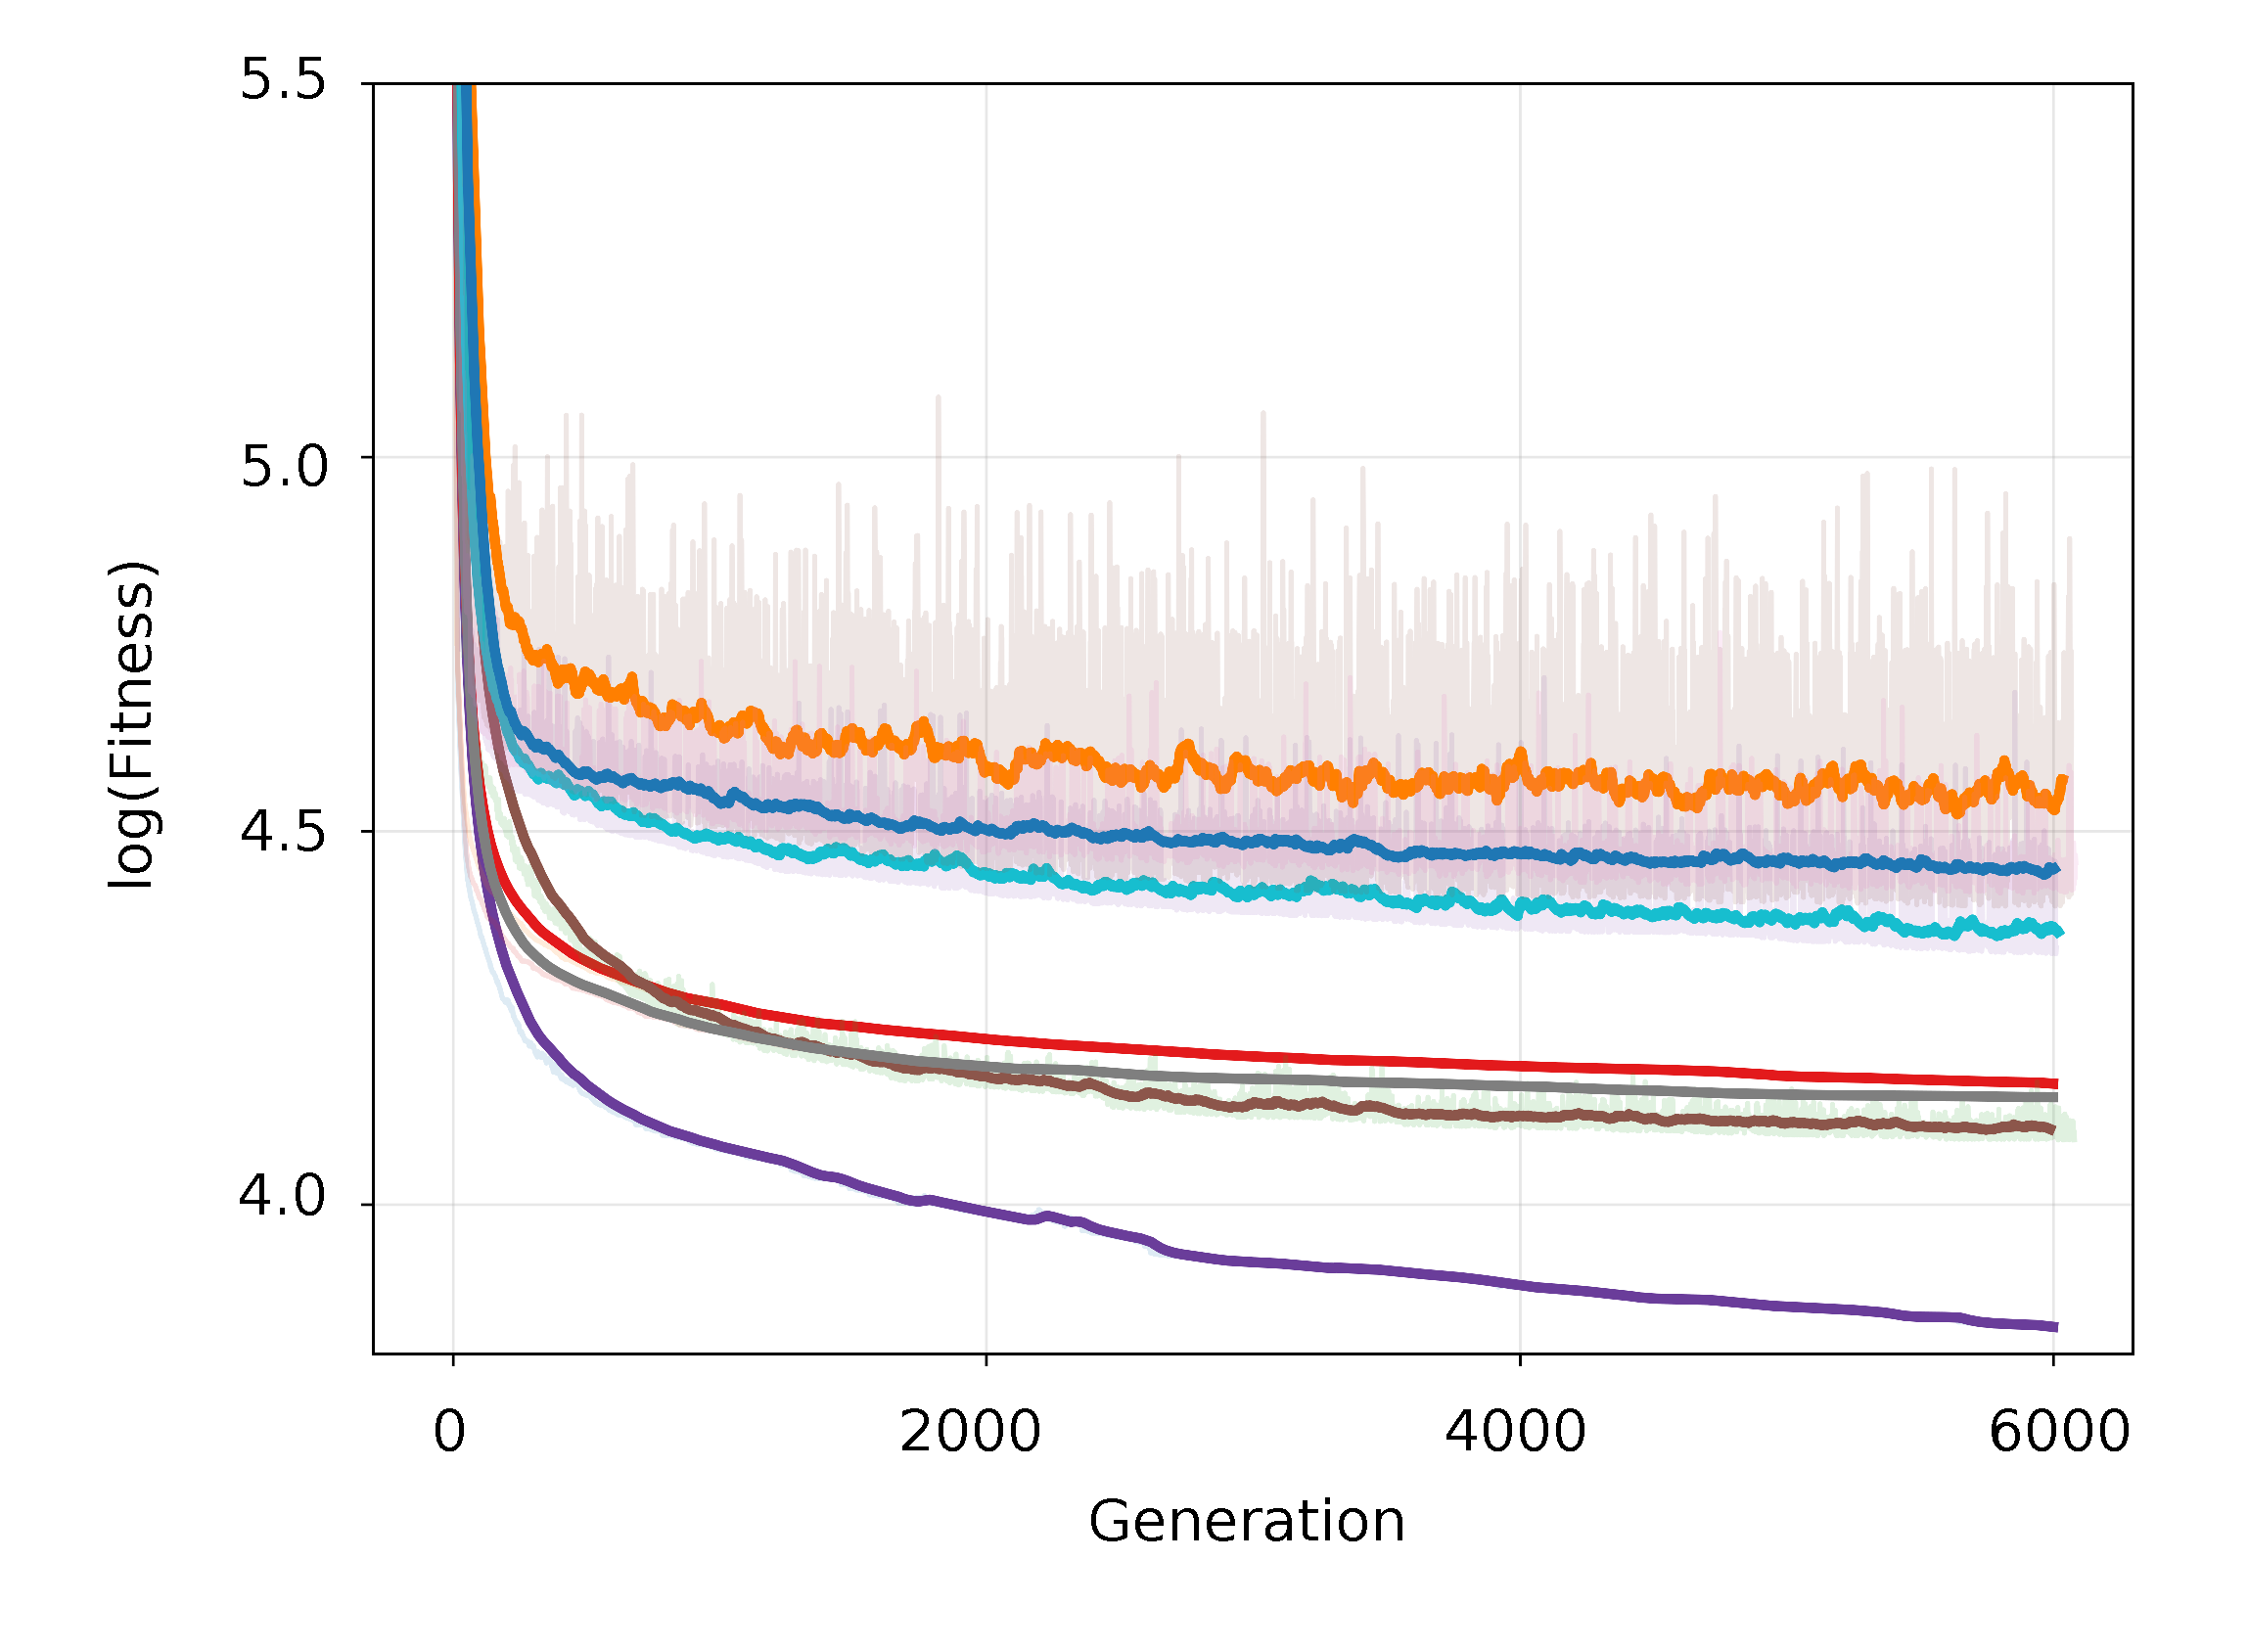
\includegraphics[width=0.82\linewidth]{images/graphcoloring_convergence_cropped.pdf}
\end{column}
\hfill
\begin{column}{0.49\linewidth}
  \centering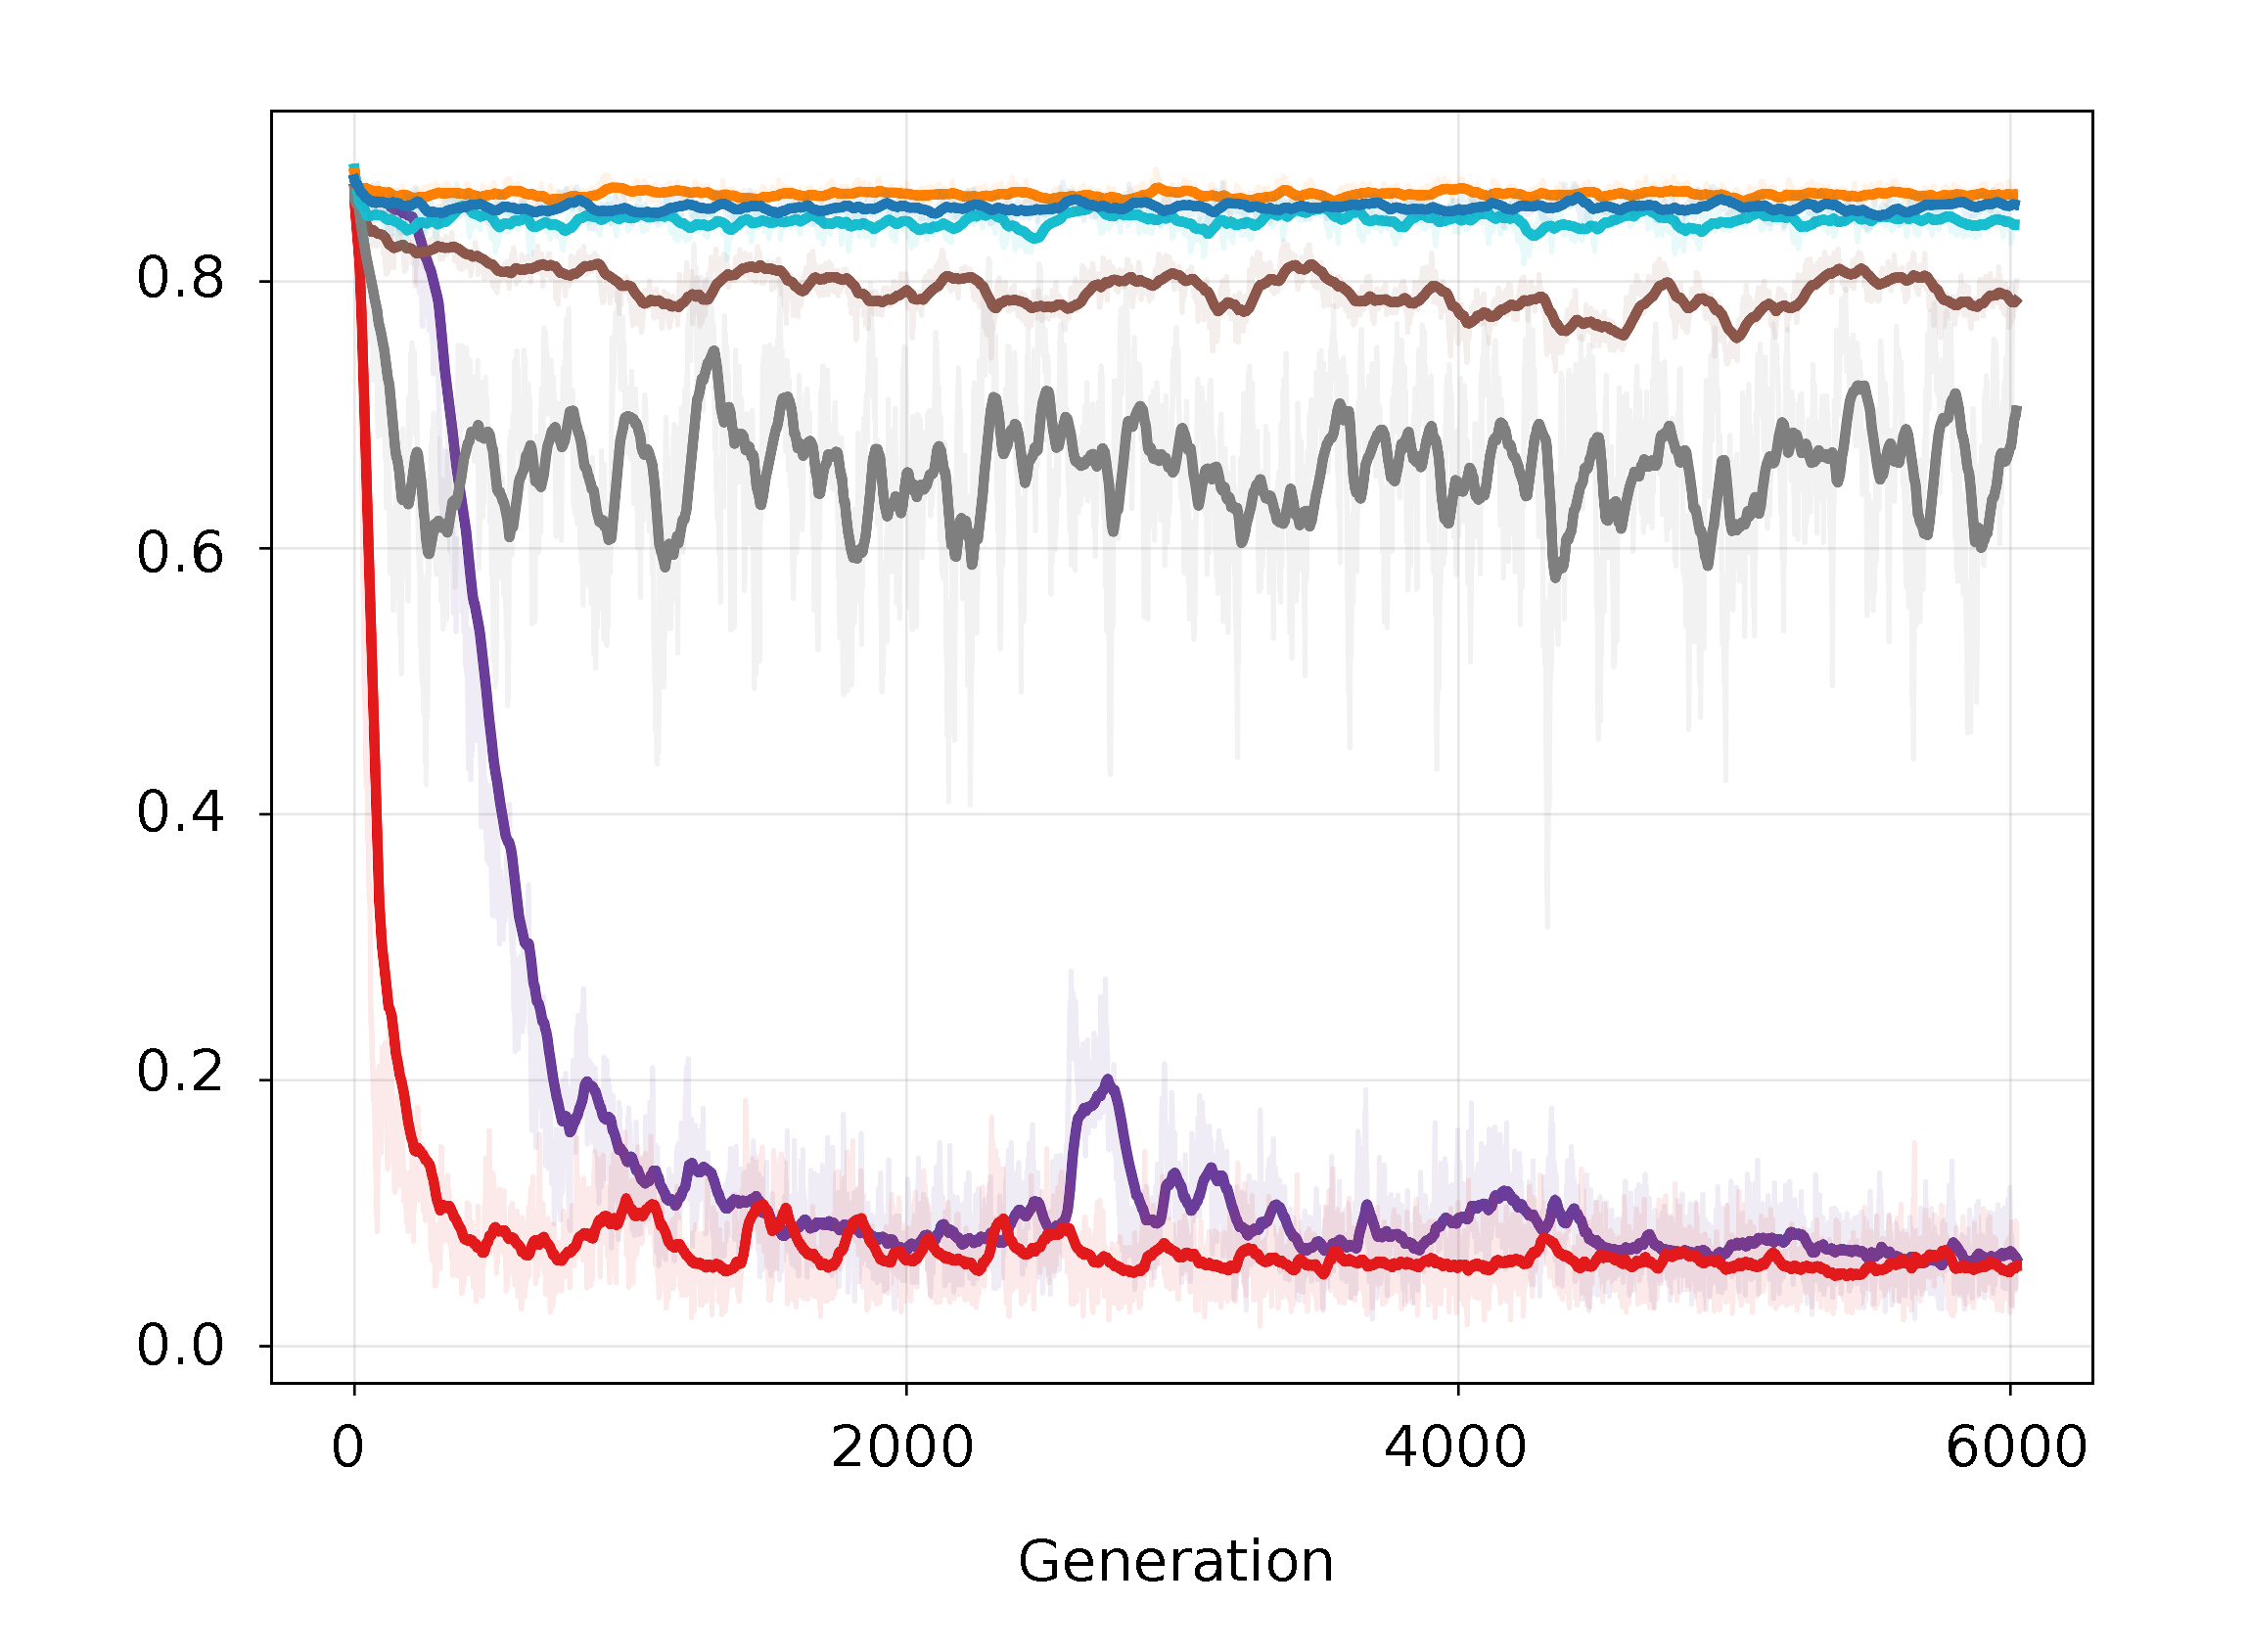
\includegraphics[width=0.82\linewidth]{images/graphcoloring_diversity_cropped.pdf}
\end{column}
\end{columns}
\vspace{2mm}

{\centering\FSNotes
\tikz[baseline=-0.6ex]\draw[colorRoulette, line width=3.5pt] (0,0) -- (0.7,0);~Roulette Wheel
\hspace{3.5mm}
\tikz[baseline=-0.6ex]\draw[colorSUS, line width=3.5pt] (0,0) -- (0.7,0);~SUS
\hspace{3.5mm}
\tikz[baseline=-0.6ex]\draw[colorLinearRank, line width=3.5pt] (0,0) -- (0.7,0);~Linear Rank
\hspace{3.5mm}
\tikz[baseline=-0.6ex]\draw[colorTruncation, line width=3.5pt] (0,0) -- (0.7,0);~Truncation
\hspace{3.5mm}
\tikz[baseline=-0.6ex]\draw[colorTournament, line width=3.5pt] (0,0) -- (0.7,0);~Tournament
\hspace{3.5mm}
\tikz[baseline=-0.6ex]\draw[colorSODGA, line width=3.5pt] (0,0) -- (0.7,0);~SODGA
\hspace{3.5mm}
\tikz[baseline=-0.6ex]\draw[colorDTS, line width=3.5pt] (0,0) -- (0.7,0);~DTS (ours)
\par}
\vspace{2mm}

\begin{columns}[t,onlytextwidth]
\begin{column}{0.48\linewidth}
  \begin{takeawaybox}
    \FSNotes\bfseries\color{bguBlue}DTS reaches lower fitness earlier and keeps improving
  \end{takeawaybox}
\end{column}
\hfill
\begin{column}{0.48\linewidth}
  \begin{takeawaybox}
    \FSNotes\bfseries\color{bguBlue}DTS maintains higher diversity than tournament
  \end{takeawaybox}
\end{column}
\end{columns}
\end{secbox}
\end{column}

\end{columns}

\sectiongap

%================================================================
% ROW 3: BOTTOM BLOCK (Scan and Contact = Conclusions)
%================================================================
\begin{columns}[t,onlytextwidth]

\begin{column}{0.370\paperwidth}
\begin{secbox}{SCAN AND CONTACT}
\vspace{2mm}
\begin{columns}[c,onlytextwidth]
  \begin{column}{0.36\linewidth}
    \centering
    \qrcode[height=5.2cm]{\projecturl}
  \end{column}
  \begin{column}{0.62\linewidth}
    \postersubsubhead{Paper \& Repo QR}
    {\color{bguMid}\FSBody\texttt{github.com/EC-KitY/DTS-for-GA}}\\[1mm]
    \FSBody\texttt{Paper, code, figures, and data.}
    \vspace{3mm}

    \postersubsubhead{Contact}
    \FSBody\texttt{\{eliads,ronedr\}@post.bgu.ac.il}\\
    \FSBody\texttt{achiya@bgu.ac.il}
  \end{column}
\end{columns}
\end{secbox}
\end{column}

\hfill

\begin{column}{0.570\paperwidth}
\begin{secbox}{8. CONCLUSIONS}
\begin{trophybox}
\centering\FSBody
\textcolor{bguMid}~~\FSNotes\bfseries\color{bguBlue}\textbf{DTS learns adaptive selection pressure, improving quality, convergence, and diversity}
\end{trophybox}
\vspace{2mm}

\begin{columns}[t,onlytextwidth]
  \begin{column}{0.24\linewidth}
    \centering\textcolor{bguMid}{\fontsize{26}{26}\selectfont\faPuzzlePiece}\\[1mm]
    {\FSSubhead\bfseries Evidence}\par\vspace{1mm}
    \FSBody DTS improves quality and convergence across benchmarks.
  \end{column}
  \begin{column}{0.24\linewidth}
    \centering\textcolor{bguMid}{\fontsize{26}{26}\selectfont\faCompass}\\[1mm]
    {\FSSubhead\bfseries Takeaway}\par\vspace{1mm}
    \FSBody Selection can be learned \textbf{online} from the evolving population.
  \end{column}
  \begin{column}{0.24\linewidth}
    \centering\textcolor{bguMid}{\fontsize{26}{26}\selectfont\faSlidersH}\\[1mm]
    {\FSSubhead\bfseries Mechanism}\par\vspace{1mm}
    \FSBody Fixed selection pressure becomes a \textbf{context-aware policy}.
  \end{column}
  \begin{column}{0.24\linewidth}
    \centering\textcolor{bguMid}{\fontsize{26}{26}\selectfont\faArrowRight}\\[1mm]
    {\FSSubhead\bfseries Next}\par\vspace{1mm}
    \FSBody Extend learned selection to richer encodings and GP.
  \end{column}
\end{columns}
\end{secbox}
\end{column}

\end{columns}

\vfill
\end{frame}
\end{document}
